\paragraph{Semantic interpretation of action-distribution change points.}
We classified the discourse function of 160 retrospectively detected
action-distribution change-point sentences and 160 same-state matched sentences while
blinding the judge to change-point status, actions, activations, and behavioral
beliefs. The primary analysis uses 152 close matched
pairs and a calibrated four-way grouping. Semantic composition did not differ
reliably between change points and matched sentences (paired permutation
$p=.219$), and adding sentence function to reasoning progress and sentence length
changed trajectory-held-out AUROC by only $+.029$ (95\% trajectory-bootstrap interval
$[-.005,+.066]$). Semantic function also did not reliably distinguish recommendation
changes, optimality losses, recoveries, or retrospective commitment onsets (smallest
corrected $q=0.406$). Thus, the detected
boundaries should be interpreted as action-routing transitions rather than as one
stereotyped verbal operation.

The positive semantic result was a difference in behavioral-belief uncertainty:
mean categorical-belief entropy was highest during route deliberation
(0.493 bits; within-trajectory permutation
$q=0.008$). In the immediate-action attention subset,
the newest-sentence attention increase was numerically largest for summaries or
restatements (0.224 percentage points per
token), although heterogeneity across semantic functions was exploratory
($p=0.053$). Finally,
7 of 18
optimality losses at primary change points occurred while all nine available
categorical belief readouts were correct at that boundary. These heterogeneous cases
are candidates for sentence deletion, replacement, and resampling interventions; they
do not by themselves establish a causal sentence mechanism.

\begin{figure}[t]
    \centering
    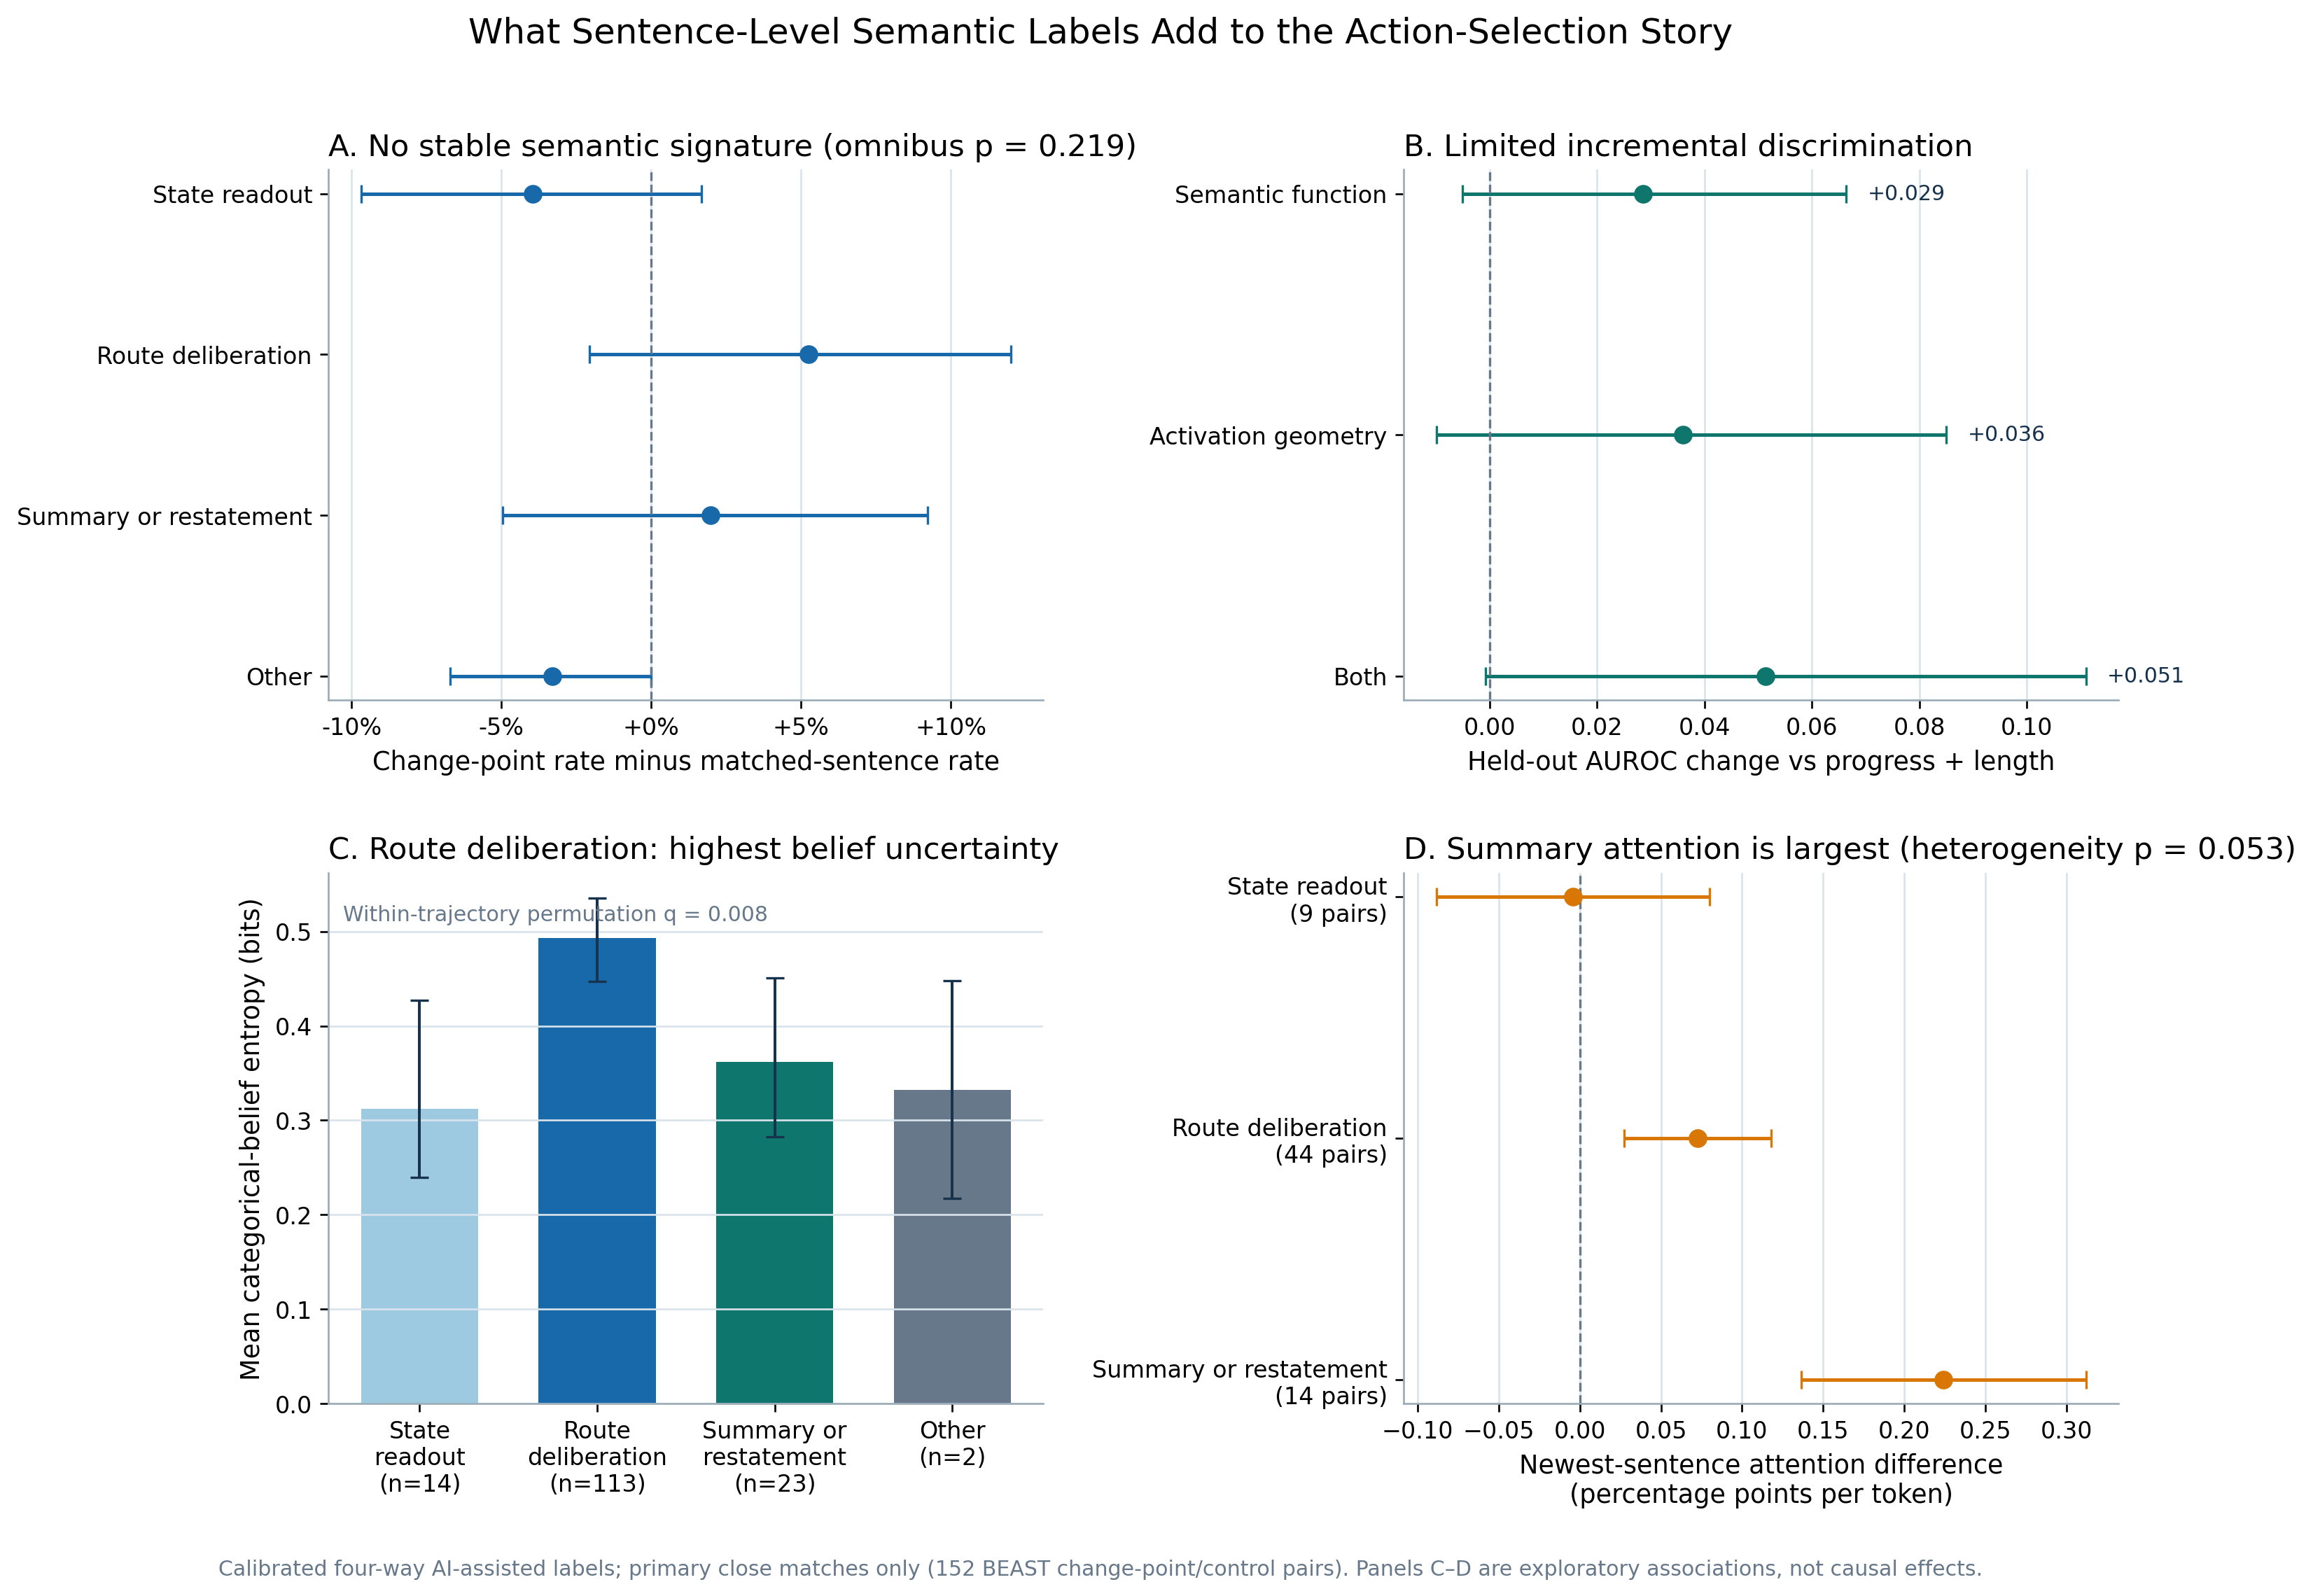
\includegraphics[width=\linewidth]{outputs/reader_facing/belief_action_reasoning_summary_v1/figs/semantic_labels_across_analyses.pdf}
    \caption{What sentence-level semantic labels add to the action-selection
    analysis. Panel A compares broad semantic-function rates in retrospective BEAST
    change-point sentences and same-state, progress- and length-matched sentences.
    Panel B reports incremental trajectory-held-out change-point discrimination.
    Panel C shows behavioral-belief entropy at change points. Panel D stratifies the
    immediate-action attention increase to the newest sentence. The four-way labels
    are calibrated AI-assisted judgments rather than human ground truth; panels C and
    D are exploratory, and all analyses are observational.}
    \label{fig:semantic_action_change_synthesis}
\end{figure}

\begin{table}[t]
\centering
\small
\begin{tabular}{p{0.25\linewidth}p{0.27\linewidth}p{0.38\linewidth}}
\toprule
Analysis & Semantic result & Implication \\
\midrule
Matched change points & No reliable four-way signature ($p=.219$) &
Do not equate a statistical change point with a correction or ``aha'' sentence. \\
Held-out discrimination & AUROC change $+.029$ $[-.005,+.066]$ &
Sentence function is not a dependable action-change monitor. \\
Exact action events & No association survives correction (minimum $q=0.406$) &
No named discourse operation reliably separates harmful changes from recoveries. \\
Behavioral beliefs & Route deliberation has highest entropy (0.493 bits; $q=0.008$) &
Semantic function identifies an uncertainty regime rather than an error regime. \\
Immediate-action attention & Summary/restatement largest; heterogeneity $p=0.053$ &
Useful for intervention prioritization, not a causal conclusion. \\
\bottomrule
\end{tabular}
\caption{Cross-analysis utility of the broad semantic-function labels.}
\label{tab:semantic_action_change_synthesis}
\end{table}
